\documentclass[a4paper,11pt]{report}
\usepackage[english]{babel}

\usepackage{graphicx}
\usepackage{cmap}
\usepackage{cite}
\usepackage[T1]{fontenc}
\usepackage{tipa}
\usepackage[utf8]{inputenc}
\usepackage{url}
\usepackage{listings}

\usepackage{amsmath}
\usepackage{amsfonts}
\usepackage{epigraph}
\usepackage{listings}
\usepackage{pgfplots}
\usepackage{tikz}
\usetikzlibrary{shapes}
\usepackage{paralist}
\usepackage{algorithm}
\usepackage{algpseudocode}
\usepackage{enumitem}

\setlength\epigraphwidth{11cm}
\setlength\epigraphrule{0pt}

\newcommand\chap[1]{%
  \chapter*{#1}%
  \addcontentsline{toc}{chapter}{\protect\numberline{}#1}}

\title{Bluetooth Qualcosa}
\author{Roberto Bampi \and Marco Dallagiacoma}

\begin{document}
	\begin{titlepage}
  \pagestyle{empty}

  \begin{center}
    {\bfseries
      \Large {\huge U}NIVERSITÀ DEGLI STUDI DI {\huge T}RENTO}

    \vspace{0.2cm}

    {\Large Dipartimento di Ingegneria e Scienza dell'Informazione}

    \vspace{0.5cm}

    \begin{center}
      
\includegraphics[width=0.3\textwidth]{img/logo_unitn.png}
    \end{center}

    \vspace{0.5cm}

    {\bfseries \Large Corso di Laurea triennale in INFORMATICA}

    \vspace{0.3cm}
    \line(1,0){338}
    \vspace{0.3cm}

    {\Large Tesi Finale}

    \vspace{2.5cm}

    {\huge \textsc{Privacy Aware Next Generation D2D Communications}\\}

    \vspace{3.0cm}

    \large
    \begin{center}
      \begin{tabular}{ccc}
        {\bfseries Relatore} &
        \hspace{5cm}
        {\bfseries Laureandi} \\

        Prof. Renato Lo Cigno &
        \hspace{5cm} Marco Dallagiacoma

      \end{tabular}
      
    \begin{tabular}{ccc}
        \hspace{10cm} Roberto Bampi

      \end{tabular}
    \end{center}
    \vspace{2cm}

    {\bfseries Anno accademico 2014-2015}
    \vfill
  \end{center}
\end{titlepage}
  	\tableofcontents
  	\chapter{Introduction}

\epigraph{``Those who would give up essential Liberty, to purchase a little temporary Safety, deserve neither Liberty nor Safety.''}{--- \textup{Benjamin Franklin} }

In the following thesis we will discuss the design and implementation of a distributed peer to peer protocol for nearby communication.
Peer-to-peer communication works by creating a network of interconnected devices that share messages between each other without relying on external infrastructure.

- external infrastructure is unreliable
-- evaluation of different peer-to-peer-tech
--- wifi-direct
--- bluetooth
--- nfc
--- wifi-infrastructure  
  	\chapter{Bluetooth}
Bluetooth is a technology that allows for short-range wireless data transmission between two or more devices, developed as a wireless alternative to common cables. The Bluetooth technology was designed to emulate cables in costs, security and capabilities. \newline
Originally developed by Ericsson, Bluetooth technology is now used in millions of devices developed by many different manufacturers.
The development of the Bluetooth technology and the licensing of the trademark are now managed by the Special Interest Group, founded in 1998 by Ericsson, IBM, Intel, Nokia and Toshiba and now consisting of more than 25000 members.
Unlike Wi-Fi, Bluetooth is designed to be energy efficient and cheap to produce. For this reason, Bluetooth is very common on portable devices like smartphones and laptops.

\section{Overview}
Bluetooth devices operate in the ISM 2.4 Ghz \cite{ISM} band, a portion of the spectrum that can be utilized without licenses.
The spectrum, from 2400 to 2483.5 MHz, is partitioned in 79 radio channels.
The radio channels start at 2402 MHz and are 1 MHz wide.
Given that the ISM spectrum is utilized by many other technologies such as 802.11g/n, cordless phones and microwave ovens, Bluetooth has been designed to be noise tolerant. 
To achieve noise tolerance Bluetooth devices switch between the 79 available channels 1600 times per second in a pseudo-random fashion. This technique is called \emph{Channel Hopping}.
Two or more devices that have the same hopping pattern share a physical channel and are considered part of the same piconet.

\subsection{Piconets}
Piconets are the most basic form of Bluetooth communication upon which all other protocols are layered on.
In a piconet a device must act as a master and all the other devices as slaves.
The physical channel is divided into slots numbered according to the Bluetooth clock of the master.
A time division duplex scheme \cite{TDD} is used to schedule access to the channel and allow master and slaves to communicate.
All the communication in a piconet is between master and slaves, there is never direct communication between slaves.

\paragraph{Addressing}
Bluetooth radios, not unlike other network cards, are supplied by the manufacturer with a 48 bit long mac address.
This address is used to determine the hopping pattern of a device and to distinguish devices during the inquiry scan phase.
Devices participating in a piconet are addressed with a 3 bit long identifier which is only valid until they are active.
This means that only 7 slaves can concurrently participate in a piconet.
The master can keep track of inactive (parked) members of a piconet using a 8 bit long identifier.

\paragraph{Scatternets}
A device may be part of more than one piconet at the same time, but can only be the master of one. This kind of set-up is called a scatternet.
At a physical level this is achieved by time-sharing access to the Bluetooth radio.

\begin{figure}[h!]
  \centering
  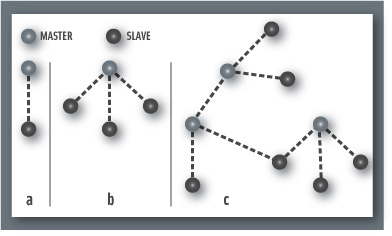
\includegraphics[width=0.7\textwidth]{img/piconets.jpg} 
  \caption{Piconets with a single slave operation (a), a multi-slave operation (b) and a scatternet operation (c).}
\end{figure}

\paragraph{Adaptive Frequency Hopping}
In a piconet the master may decide to alter the hopping sequence to only use a subset of the available 79 channels. The master will exclude  noisy channels and then communicate the new hopping pattern to all the slaves.

\subsection{Connection setup}
A connection is normally created following two steps: inquiry and page.
The inquiry scan is necessary to discover the mac addresses of devices that are in range and the paging procedure is used to establish the actual connection.
In the inquiry phase the source sends out inqury packets and then listens for inquiry reply.
If a listening device is in the inquiry phase it can receive and reply to such packets.
After the inquiry scan is complete a paging procedure can be started to establish the connection.
The device which starts the paging procedure will become master of the piconet formed as a result.

\subsection{Range}
Bluetooth divides devices into three classes based on how much transmission power they have, the transmission power influences the distance 

\vspace{0.3cm}
\begin{tabular}{|c|r|r|}
 \hline
 class & transmission power output & range \\ \hline
 1 & 100 mW & 100 meters \\
 2 & 2.5 mW & 10 meters \\
 3 & 1 mW & 1 meter \\
 \hline
\end{tabular}
\vspace{0.3cm} 

\noindent
Most modern smartphones are class 2 devices

\subsection{Baseband}
The \emph{baseband} \cite{baseband} implements the medium access control and physical layer parts of the Bluetooth system.
It manages physical channels and links, hop selection and scanning for nearby devices (inquiry scan).


\section{Bluetooth Architecture}
The Bluetooth technology is divided into two specifications: the core and the profile specifications. The core specification defines how the technology works, while the profiles define how to leverage on the core technologies to build a Bluetooth application.
The Bluetooth core system consists of an RF transceiver, the baseband, and a set of protocols.

\begin{figure}[ht!]
  \centering
  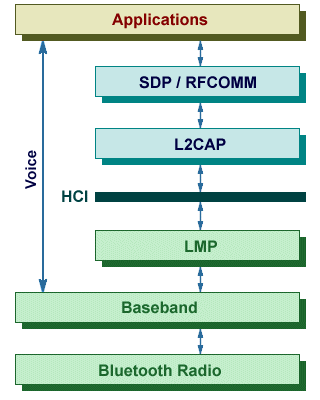
\includegraphics[width=0.3\textwidth]{img/bluetooth_protocol_stack.png} 
  \caption{The Bluetooth protocols stack}
\end{figure}

\subsection{L2CAP}
The L2CAP (Logical Link Control and Adaptation Layer) layer provides both connectionless and connection-oriented services to higher level protocols. Its tasks include multiplexing of protocols (since Baseband does not contemplate a "type" field to specify the kind of protocol that generated a package), segmentation and reassembly of PDUs (Protocol Data Unit), and QoS (Quality of Service) support.
L2CAP enables higher level applications and protocols to send and receive L2CAP data packets up to 64 kilobytes in length.

The L2CAP layer provides logical channels, named L2CAP channels, which act as a logical connection on top of a baseband connection.
More channels can rely on the same baseband connection.
An endpoint of an L2CAP channel is identified by a channel identifier (CID).

By default, L2CAP uses ACL as the transmission link.

\subsubsection{ACL}
Bluetooth supports two main types of connection links: ACL (Asynchronous Connection Less) and SCO (Synchronous Connection Oriented).
The most widely used one is ACL, which garantees that data is delivered and in the correct order and without errors.

ACL links can operate both in a symmetric and in a asymmetric mode, and can be granted a Quality of Service by setting the appropriate channel parameters during connection.

\subsection{RFCOMM}
The RFCOMM protocol \cite{RFCOMM} emulates the capabilities of the RS-232 serial ports over the L2CAP protocol. It was developed to make it easier for manufacterers to use the Bluetooth technology in their existing applications. Similarly to TCP, RFCOMM provides applications a simple point-to-point reliable data stream, supporting multiplexing and flow control between devices and applications.

It is possible to maintain up to 60 simultaneous connections between two devices (each one can initialize up to 30 connections with the other one) using RFCOMM, while the maximum number of open simultaneous connections on a single device is implementation-specific.

Excluding Bluetooth LE (Low Energy), RFCOMM is the only Bluetooth protocol officially supported by the Android API.

\subsection{SDP}
The Service Discovery Protocol (SDP) enables Bluetooth devices to discover the existence and the attributes of services provided by other server applications.
SDP provides the ability for clients to search for needed services based on specific attributes of those services. 
However, it is possible to retrieve a list of all services with their attributes from another device.
This process is called browsing.

While SDP provides the means to discover services it does not provide a mechanism to utilize them.

SDP is bound to the L2CAP protocol.

\paragraph{Service Record}
All of the information about a service is stored by the SDP server as a single service record, which consists in a list of attributes.
Each attribute represent a characteristic of the service, such as the name or the UUID. Each attribute is stored as a ID-VALUE pair, where the ID is a 16 bit unsigned integer and the value is a variable length field.
  	
\subsection{Benchmark Application}
All of the benchmarking code was implemented in a standard android application which is available on Github \cite{benchmarking-code}.
The application was responsible for running a simulation and collecting the relevant metrics for each simulation scenario.
To allow programmatic access to all this functions, a small HTTP server \cite{nanohttpd} was embedded into the application.
This approach allowed manual testing of the functionality during development as well as allowing a remote script to run the real simulations.
Three endpoints were exposed on the HTTP server by the application; one to get the Bluetooth name and MAC address of the device and two to run simulations.

A python script was developed to run the individual simulations, collect and plot the data generated in the process.
The script used the list of local IP addresses as input and collected all of the necessary information via the \texttt{/mac} HTTP endpoint on each device.


The second benchmark was designed to test the performance of a device to send multiple messages to a variety of other devices.
For this test a single device, the master, sent a predefined number of messages to a set of devices.
When the devices received a message they sent a reply back so that the master could compute the round-trip-time.

To initiate the test the script invoked the \texttt{/messages} endpoint on the master device, passing a list of targets and the number of messages to send to each client as query string parameters.

Each message sent by the master was tagged with a random UUID, so when the response was received, the master was able to compute the round trip time for that message.
Once the master received a response for every request sent (or after the timeout went off), a CSV was returned as response to the HTTP request.
This CSV contained six fields: ``to'', ``from'', ``message\textunderscore size'', ``started'', ``received'' and ``finished''.
``to'' and ``from'', like in the previous test, contained the Bluetooth MAC address of client and server.
``message\textunderscore size'' contained the size of the messages sent (1024 bytes by default).
``started'' and ``stopped'' were timestamps mesured when the mesage was sent and a reply was received, completing the round-trip.


\subsubsection{Technical details}The test begins when the master receives a HTTP GET request to the endpoint relative to the test, specifying parameters like order of the devices in the ring, number of rounds and size of payload. The master then creates a token, assigning to it a unique uuid that will identify that run of the test, and returns the uuid as the HTTP response.
In order to enable the master to inform the peers about the configuration of the test, the information required is embedded in the token, that is subsequently passed between the devices.
The master starts the process by sending a ping to the next device. Once it receives a pong (an acknowledgement), it sends the token to the next devices and waits until it receives the token again. 
This process is repeated by every peer in the ring, as described in Algorithm \ref{pseudo:ring_peer}.
When the master receives the token again, it saves the measurements taken locally (removing them from the token, thus preventing the token from becoming too large) and, if the desired number of rounds have been completed, stops the loop by not forwarding the token again to the following device.
Results can then be retrieved by making a HTTP request to the master of the ring and specifying the UUID of the desired run of the test.


  	\chapter{Analysis of alteratives}
\section{Firechat}
Firechat is a proprietary chat software available for iOS and Android devices.
It is developed by OpenGarden \cite{opengarden}, a company specialized in the creation of peer-to-peer technology.
One of the features of Firechat is the ability to communicate with nearby devices in order to exchange messages in the absence of an Internet connections.
\textbf{Note}: we only tested the Android version of the application.

\paragraph{Nearby Communication} In addition to the various chatrooms available on OpenGarden's servers, Firechat has a ``Nearby'' chatroom that is used to communicate directly with other devices.
In order to spread messages into the ``Nearby'' chatroom the application leverages a combination of communication methods including: UDP broadcast, Bluetooth RFCOMM, Bluetooth Low Energy (BTLE) \cite{btle} and WiFi Direct \cite{wifi-direct}.
Messages sent in the ``Nearby'' chatroom are received by everyone else.

\subsection{Analysis}
Since the source code for the program was not available, some analysis were performed in order to infer the behavior of the application.

\paragraph{Black box testing}
In the first experiment a copy of the Firechat application was downloaded from the Google Play Store \cite{google-play-store} and installed on three devices.
Cellular and WiFi connections were turned of while Bluetooth was enabled.
Manual pairing was performed on all three devices (each of them was paired with the other two) and then the application was open.
After a couple of minutes where the messages each phone sent were not received by the other two, the three devices connected in a master-slave setup.
One of the three devices (``A'') received messages sent from the other two (``B'' and ``C'') and was able to send messages to both.
Messages sent by ``B'' were only received by ``A'' but never by ``C'' and vice versa.
Any attempt to connect more devices to the chatroom proved unsuccessful.
This test proved that while a possible communication channel between ``B'' and ``C'' was available through ``A'' the application was not able to exploit it to relay messages.


We describe two experiments we performed that, along with the information described in \cite{firechat-analysis-1} \cite{firechat-analysis-2} allowed us to draw the conclusions above.

\subsection{Pitfalls}
Even though the application allows some form of local communication it has several problems that make it unfit for a context where discretion is important [todo: add reference to article about afghanistan].

\subsubsection{Cleartext protocol}
First and foremost all of the messages sent through the application are not encrypted in any way: the payload is a json \cite{json} object with the username and the message as keys.
This makes it trivially easy for an attacker to intercept and tamper messages.
Additionally if the recipient receives a message it has no way to verify its origin. This is true for both local (``Nearby'') and remote communication.

\subsubsection{Single hop communication}
When a device running Firechat receives a connection (on RFCOMM or Wifi-Direct) it sends to the newly connected peer the last 5 messages it sent to the ``Nearby'' room. It does not, however, re-send messages it received from its neighbors. This means that if a device ``A'' sends a message to device ``B'' and device ``B'' later encounters ``C'', ``C'' will not be able to know what ``A'' said (but it will receive the last 5 messages sent by ``B'').
[INSERISCI GRAFICO QUI]



  	\bibliographystyle{unsrt}
  	\bibliography{biblio}
\end{document}